\section{Review and Retrieval in the Interface}
\label{app:interface-details}
\suppressfloats[t]
\subsection{Campaign Archive and Review Interface}
\label{sec:interface}
\label{sec:retrieval}
The browser and command-line interface retrieve checks, evidence, and decisions from the same persistent campaign archive~\cite{scpCheckpoint}. From a run, an engineer can locate the failed check, verify the evidence fingerprint, and follow links to the reviewer, rationale, and decision time. The examples below show an approved scope change, the retained failure, and the corresponding retrieval commands.


\paragraph{Earlier budget authorization}
\label{sec:review-example}
\label{sec:budget-example}
The earlier 14M campaign allowance provides a concrete authorization example. Its request asks: ``Approve 60 minutes and up to 2M accounted tokens within the existing 14M ceiling, retaining prior charges and the documented best-effort/1M unmetered-failure debit policy?'' The requested 2M allowance remains within the cumulative 14M ceiling. If $u$ tokens are already accounted for, full use requires $u+2\mathrm{M}\leq14\mathrm{M}$; reservations further reduce the available balance.

The \texttt{Campaign} service records extensions against the prior allowance or deadline and preserves consumption. The 1M debit estimates usage when measurement is unavailable. Approval must be recorded separately from this request. The recorded name attributes approval; identity authentication remains external to this record~\cite{scpCheckpoint}.

\paragraph{Scope review}
In the synthetic case in Figure~\ref{fig:ui-approval-summary}, A passed and B failed. Approving B's exclusion enabled partial acceptance while retaining the failure, rationale, revisit condition, and option to revoke it. The excluded obligation receives no verification credit. The interface's separate \emph{Defer selected} action keeps B required.

\begin{figure}[!htbp]
\centering
% Print-sized excerpts from the same unedited application capture.
\begingroup
\setlength{\fboxsep}{4pt}
\setlength{\fboxrule}{0.4pt}
\fcolorbox{black!35}{black!3}{%
\begin{minipage}{\dimexpr\linewidth-2\fboxsep-2\fboxrule\relax}
\small\color{black}
\textbf{(a) Verification status and evidence link}
\par\vspace{2pt}
\centering
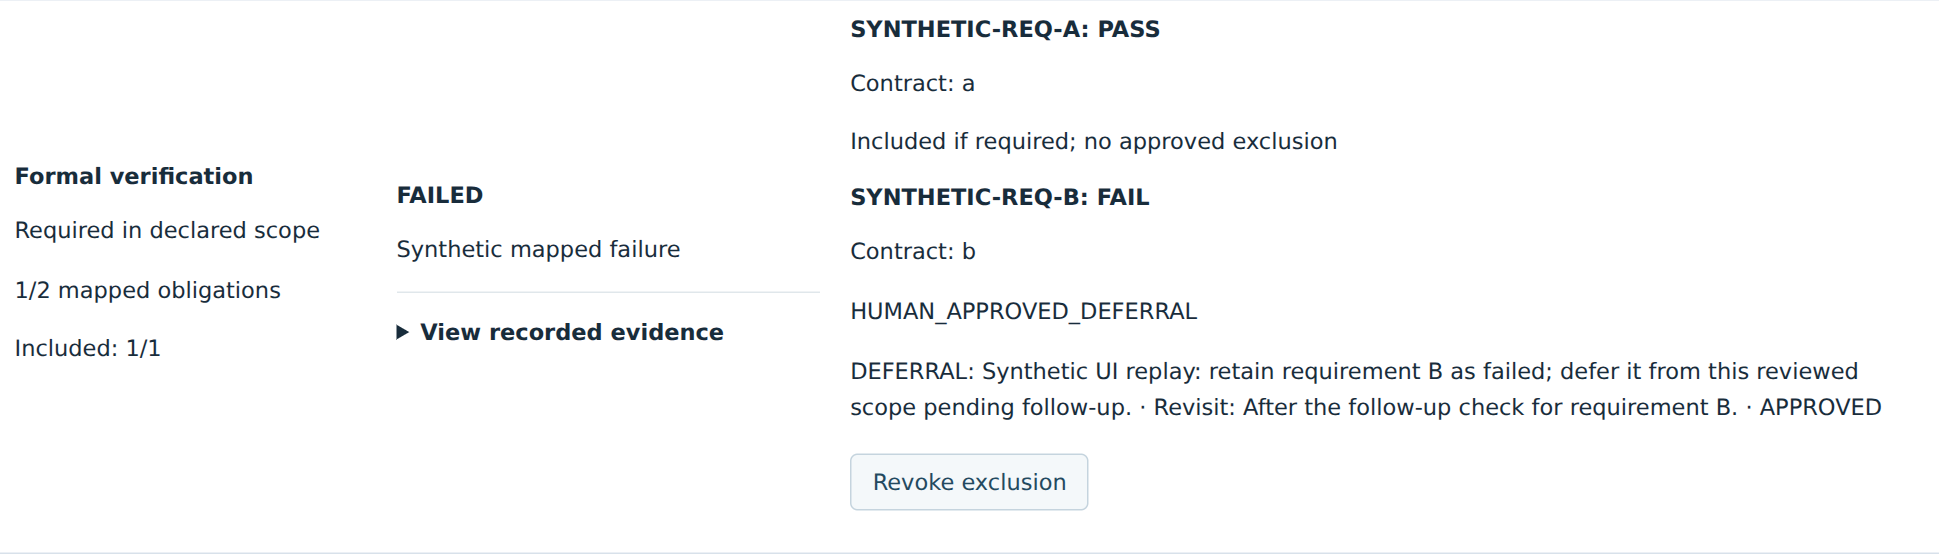
\includegraphics[width=.82\linewidth,trim=0bp 170bp 1115bp 150bp,clip]{assets/ui-approval-accepted.png}
\par\vspace{5pt}
\raggedright
\textbf{(b) Per-requirement results and approval}
\par\vspace{2pt}
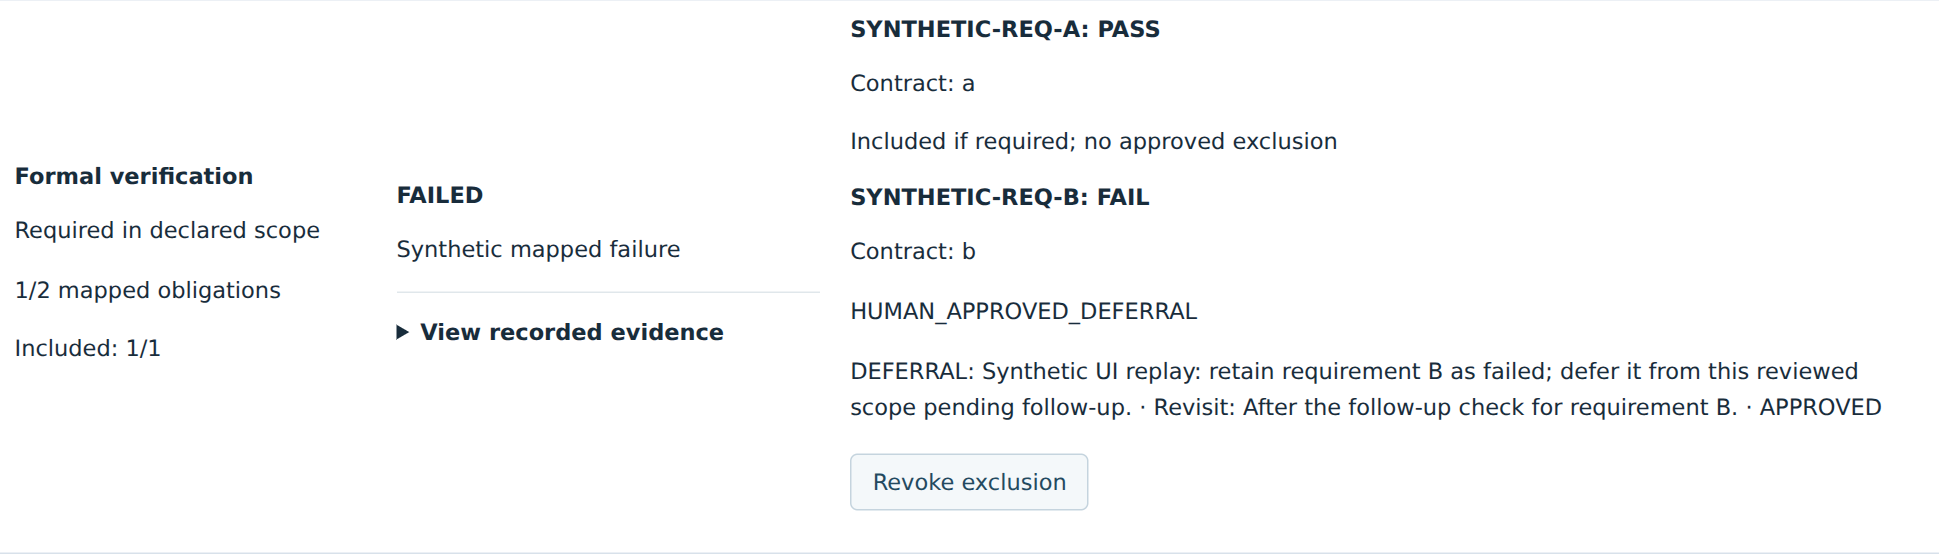
\includegraphics[width=\linewidth,trim=830bp 31bp 10bp 0bp,clip]{assets/ui-approval-accepted.png}
\end{minipage}%
}
\endgroup

\caption{Review of a synthetic case in the workbench. An approved exclusion leaves one passing obligation in scope (1/1). The original result still shows a failure and 1/2 mapped obligations. The review panel retains the rationale and revisit condition. The evidence link opens the original result.}
\Description{Two excerpts from the browser interface. The verification summary shows a failed check, one of two mapped obligations, one of one included obligations, and an evidence link. The review panel shows A passing and B failing with a human-approved exclusion, its rationale and revisit condition, and a revoke control.}
\label{fig:ui-approval-summary}
\end{figure}

\subsection{Retrieval Commands}
For that case, let $R$ be run \texttt{a83f146e}\ldots, $H$ evidence fingerprint \texttt{3db914d832ff}\ldots, and $P$ request \texttt{610bd646}\ldots. With \texttt{./scp-workbench --state-dir STATE}, the schematic queries are
\begin{quote}\small\ttfamily
trace R\\
trace R --evidence H\\
approval P
\end{quote}
The trace identifies the failed check and $H$. The second query retrieves the A-pass/B-fail evidence and checks its SHA-256. The review record links it to B's exclusion and request $P$; the third query retrieves approval, reviewer label, and decision time. A separate acceptance record binds the review fingerprint. The original trace remains \texttt{FAILED}.

Signed export uses a bundle location and the expected policy and trusted keys. Three pilot cases check retention across clean service reopening (Section~\ref{sec:evaluation}); browser-restart behavior remains untested~\cite{scpCheckpoint}.
